\documentclass[10pt]{article}

\usepackage{mathtools}
\usepackage{amsmath}
\usepackage{amssymb}
\usepackage{color}
\usepackage{fullwidth}
\usepackage{graphicx}
\usepackage[margin=0.6in]{geometry}
\usepackage{tikz}
\usepackage{float}
\usepackage[hidelinks, urlcolor=blue, linkcolor=blue, colorlinks=true]{hyperref} 

\DeclarePairedDelimiterX\set[1]\lbrace\rbrace{\def\given{\;\delimsize\vert\;}#1}

\newcommand{\bcent}{\begin{center}}
\newcommand{\ecent}{\end{center}}
\newcommand{\tb}{\textbf}
\newcommand{\noin}{\noindent}
\newcommand{\benum}{\begin{enumerate}}
\newcommand{\eenum}{\end{enumerate}}
\newcommand{\bitem}{\begin{itemize}}
\newcommand{\eitem}{\end{itemize}}
\def\boxx#1{
    \framebox{
    \begin{tabular}{c}
    \\[-1pt]
    #1 \\
    \\[-1pt]
    \end{tabular}
    }
}

%%% This command makes a framed box of a chosen height.
\newcommand{\makenonemptybox}[2]{%
\par\nobreak\vspace{\ht\strutbox}\noindent
\setlength{\fboxrule}{0pt} % set this to 0pt to make invisible
\fbox{%
\parbox[c][#1][t]{\dimexpr\linewidth-2\fboxsep}{
  \hrule width \hsize height 0pt
  #2
 }%
}%
}
\makeatother    


\begin{document}

{\bcent\fontfamily{cmss}\selectfont
\begin{tabular}{c}
\textbf{}~~~~~~~~~~~~~~~~~~~~~~~~~~~~~~~~~~~~~~~~~~~~~~~~~~~~~~~~~~~~~~~~~~~~~~~~~~~~~~~~~~~~~~~\textbf{{\color{red} Due}: 11:59pm Sunday January 28, 2024}\\\hline
\end{tabular}\ecent
}

{\fontfamily{cmss}\selectfont
\large\bcent\tb{}\\
\tb{}\\
\vspace{0pt}
%\tb{Term Test 1}\\

\tb{\Large MAT185 Linear Algebra}\\

\tb{Assignment 1}
\ecent}



\noin{\fontfamily{cmss}\selectfont\tb{\large Instructions:}} \\ %% Fairly standard and designed to save time; however, tweak as necessary.

\noindent Please read the {\bf MAT185 Assignment Policies \& FAQ} document for details on submission policies, collaboration rules and academic integrity, and general instructions. 

\benum


\item {\bf Submissions are only accepted by} \href{https://www.gradescope.ca}{Gradescope}. Do not send anything by email.  Late submissions are not accepted under any circumstance. Remember you can resubmit anytime before the deadline. 

\item  {\bf Submit solutions using only this template pdf}.  Your submission should be a single pdf with your full written solutions for each question. If your solution is not written using this template pdf (scanned print or digital) then your submission will not be assessed. Organize your work neatly in the space provided.  Do not submit rough work. 

\item  {\bf Show your work and justify your steps} on every question but do not include extraneous information.  Put your final answer in the box provided, if necessary.  We recommend you write draft solutions on separate pages and afterwards write your polished solutions here on this template.

\item  {\bf You must fill out and sign the academic integrity statement below}; otherwise, you will receive zero for this assignment. 


\eenum

\vspace{30pt}


\noin{\fontfamily{cmss}\selectfont\tb{\large Academic Integrity Statement:}} \\

%%% Student information

% Student 1
\fbox{
\begin{minipage}{\textwidth}
{
\vspace{0.2in}

\makebox[\textwidth]{\sffamily Full Name:\enspace\hrulefill}

\vspace{0.2in}

\makebox[\textwidth]{\sffamily Student number:\enspace\hrulefill}

\vspace{0.1in}
}
\end{minipage}
}

\vspace*{0.1in}

% Student 2
\fbox{
\begin{minipage}{\textwidth}
{
\vspace{0.2in}

\makebox[\textwidth]{\sffamily Full Name:\enspace\hrulefill}

\vspace{0.2in}

\makebox[\textwidth]{\sffamily Student number:\enspace\hrulefill}

\vspace{0.1in}
}
\end{minipage}
}
~

I confirm that:

\begin{itemize} 
	\item I have read and followed the policies described in the document {\bf MAT185 Assignment Policies \& FAQ}.
	\item In particular, I have read and understand the rules for collaboration, and permitted resources on assignments as described in subsection II of the the aforementioned document. I have not violated these rules while completing and writing this assignment. 
	\item I understand the consequences of violating the University's academic integrity policies as outlined in the \href{http://www.governingcouncil.utoronto.ca/policies/behaveac.htm}{Code of Behaviour on Academic Matters}. I have not violated them while completing and writing this assignment.
\end{itemize}
By signing this document, I agree that the statements above are true. 

% You should sign this PDF after compiling. Do not write your signature using LaTeX.
\vspace{0.2in}
{\large 
\makebox[\textwidth]{\sffamily Signatures: 1)\enspace\hrulefill} 

\vspace{0.2in}

\makebox[\textwidth]{\sffamily \hspace*{20mm} 2)\enspace\hrulefill} 

}

\vfill


\pagebreak

%%% Questions

\noin{\bf 1.}   A {\it \color{red} vector spyce} is a set $V$  together with two operations called {\it vector addition} and {\it scalar multiplication} such that the following nine {\it axioms} hold: 

\begin{itemize}
\item[ (i)]  For all vectors ${\bf x,y} \in V$, ${\bf x+y} \in V$



\item[(ii)]   For all vectors ${\bf x, y, z} \in V$, $\bf{(x+y)+z}=\bf{x+(y+z)}$

\item[(iii)]   There exists a vector ${\bf 0}\in V$ with the property that  $\bf {x+0}=\bf {x}$ for all vectors ${\bf x}\in V$

\item[(iv)]    For each vector ${\bf x}\in V$, there exists a vector $-\bf{x} \in V$ with the property that $\bf x + (-x)=0$

\item[(v)]  For all vectors ${\bf x}\in V$, and scalars $c\in \mathbb R$, $c{\bf x} \in V$

\item[(vi)]   For all vectors ${\bf x} \in V$, and scalars $c, d\in \mathbb R$, $(cd){\bf x}=c(d{\bf x})$

\item[(vii)]  For all vectors ${\bf x, y} \in V$, and scalars $c\in \mathbb R$, $c({\bf x+y})=c{\bf x}+c{\bf y}$

\item[(viii)]  For all vectors ${\bf x} \in V$, and scalars $c, d\in \mathbb R$, $(c+d){\bf x}=c{\bf x}+d{\bf x}$

\item[(ix)]  For all vectors ${\bf x} \in V$, $c{\bf x}={\bf 0}$ implies that either $c=0$ or ${\bf x}={\bf 0}$

\end{itemize}
\vspace{20pt}




\noin  Prove that a {\it \color{red} vector spyce} is a vector space.


%Question 1

{
	\vspace*{-10pt}
	%%% Do not change the height of this box. Your work must fit inside it.
	
	\makenonemptybox{450pt}{  
	
	%%% Your work goes here! 

	}
}


\pagebreak 


\noin {\bf 2.}  Let $V=\{ a_0+a_1x+a_2x^2 \mid a_0>0 \}$.  Define vector addition in $V$ by 
$$(a_0+a_1x+a_2x^2)+(b_0+b_1x+b_2x^2) = (a_0b_0)+(a_1+b_1+4)x+(a_2+b_2)x^2$$
and scalar multiplication in $V$ by
$$c(a_0+a_1x+a_2x^2) = a_0^c+(ca_1+4(c-1))x+ca_2x^2$$

\vspace{20pt}
\noin Verify that axiom MIII. (Medici, pp104) holds in $V$.

%Question 2
{
	\vspace*{-10pt}
	%%% Do not change the height of this box. Your work must fit inside it.
	
	\makenonemptybox{550pt}{
	
	%%% Your work goes here! 

	}
}   








\pagebreak

 \noin{\bf 3.}  We asked ChatGPT if $V=\{ f \mid f' \mbox{ is constant} \}$ is a vector space.  It's response is given below.\\

\begin{center}
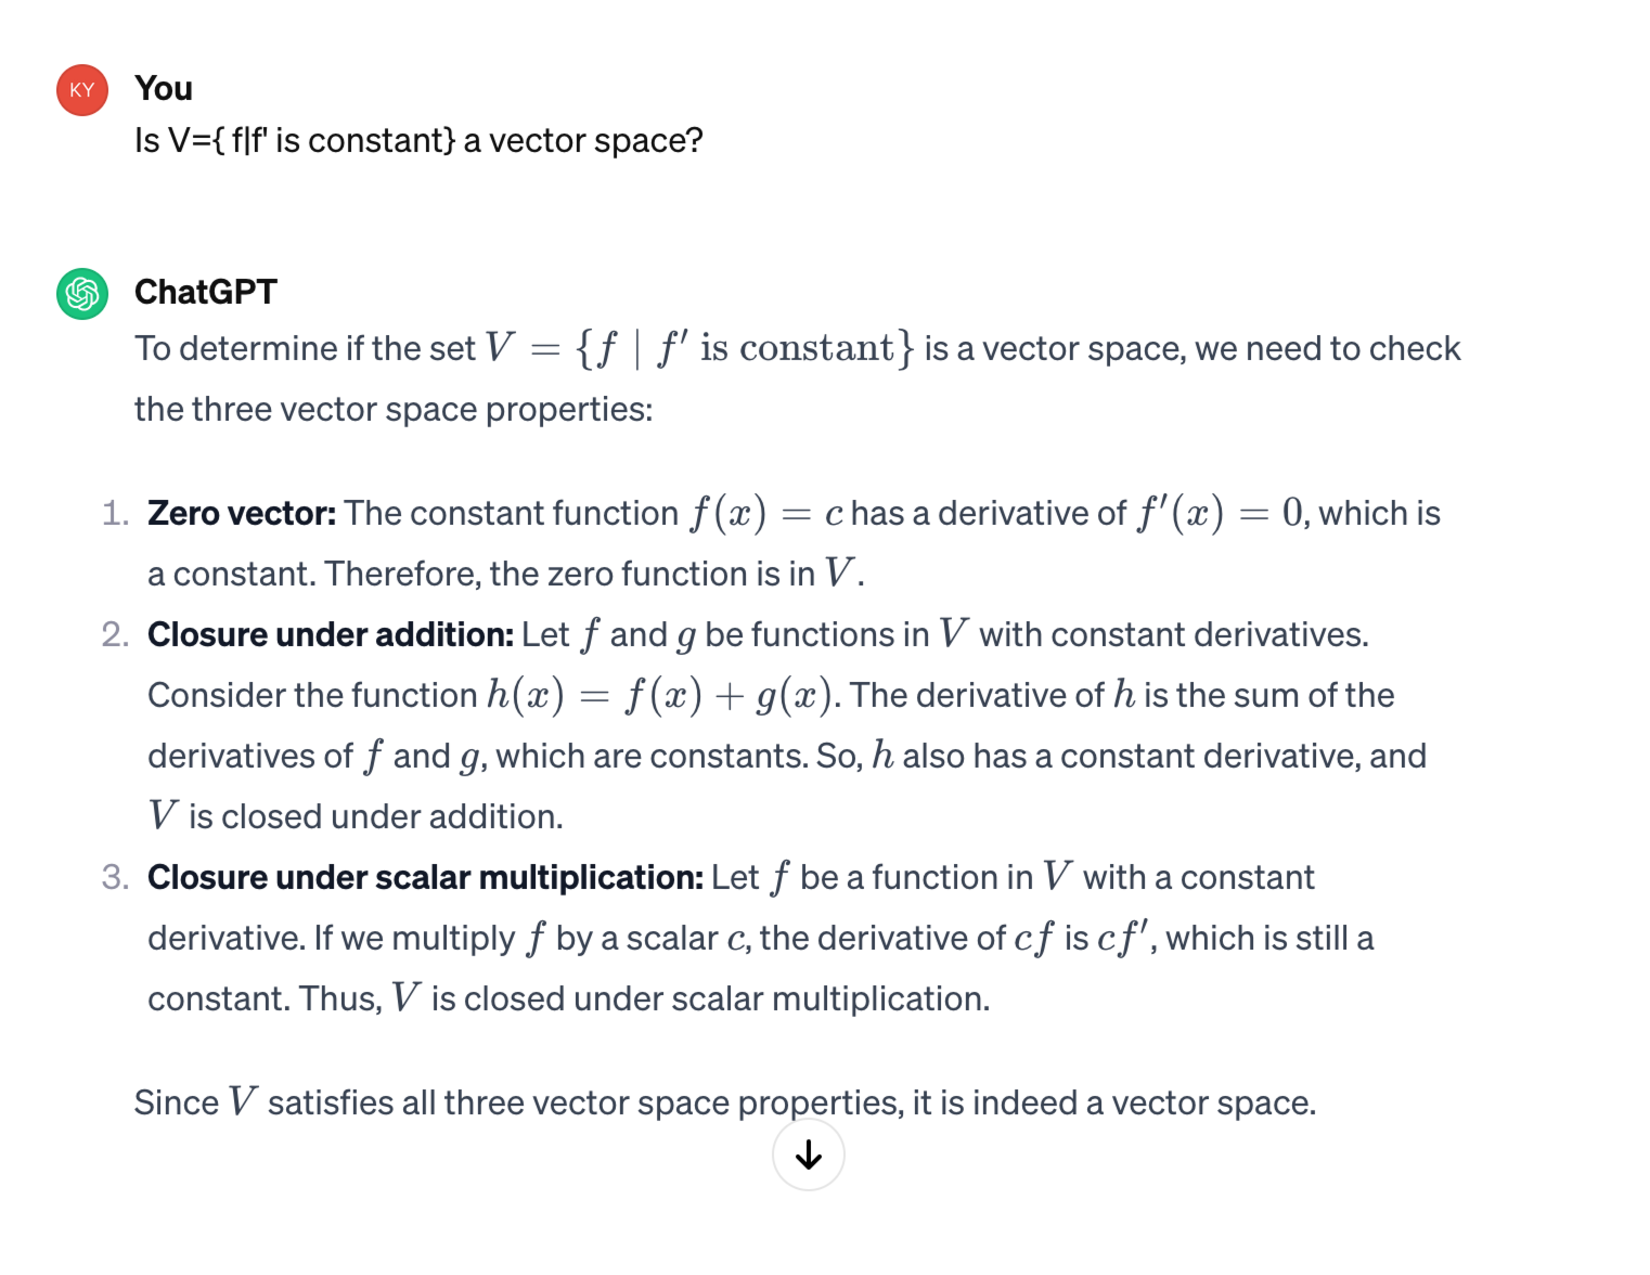
\includegraphics[width=.8\textwidth]{185A1Chat.pdf}
\end{center}

\noin Identify {\it two} errors in ChatGPT's response and write {\it two} paragraphs, one for each error, each of which clearly identifies an error, and how you would correct them.


%Question 3

{
	\vspace*{-10pt}
	%%% Do not change the height of this box. Your work must fit inside it.
	
	\makenonemptybox{275pt}{ 
	
	%%% Your work goes here! 

	}
}







\pagebreak

\noin{\bf 4.}  Let $c\in \mathbb R$, and consider the subset $W_c=\{\, (x, y, z) \in \mathbb R^3 \, \mid  \, x+y+z=c \left | z \right | \, \}$ of $\mathbb R^3$.  Determine {\it all} values of $c$ such that $W$ is a subspace of $\mathbb R^3$.  Your answer should clearly demonstrate that you've found {\it all} values of $c$ such that $W_c$ is a subspace.  This includes  demonstrating  why $W_c$ is not a subspace for certain values of $c$, if you think no such $c$ exists.

%Question 3

{
	\vspace*{-10pt}
	%%% Do not change the height of this box. Your work must fit inside it.
	
	\makenonemptybox{550pt}{
	
	%%% Your work goes here! 

	% mistake 1: chatgpt assumed that V is a subset of a vector space, but did not state why
	% mistake 2: chatgpt got the zero vector wrong

	}
}

\end{document}
